\chapter{Results and Analysis}
\label{chap:results}

Two evaluation settings: synthetic (controlled, 300 queries from the same DEM) and real-photo (68 Google Street View panoramas from Khumbu).

\section{Synthetic Evaluation}

\subsection{Setup}

300 synthetic query images rendered from the Copernicus GLO-30 DEM under different weather and lighting. Ground truth is the known camera location.

\begin{table}[H]
\centering
\caption{Synthetic evaluation setup}
\label{tab:evaluation_setup_results}
\begin{tabular}{ll}
\toprule
\textbf{Parameter} & \textbf{Value} \\
\midrule
Study area & Khumbu, Nepal \\
Reference viewpoints & 4{,}920 (500\,m grid) \\
Queries & 300 \\
Ground truth & Camera location \\
\bottomrule
\end{tabular}
\end{table}

\subsection{Query Images}

Rendered under different weather and lighting conditions.

\begin{figure}[H]
\centering
\begin{subfigure}[b]{0.82\textwidth}
\centering
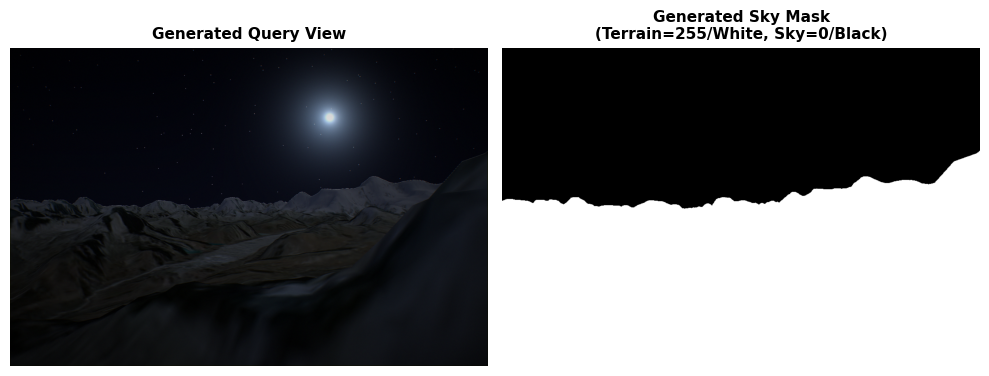
\includegraphics[width=\textwidth]{src/images/synthetic.png}
\end{subfigure}

\vspace{0.5em}

\begin{subfigure}[b]{0.82\textwidth}
\centering
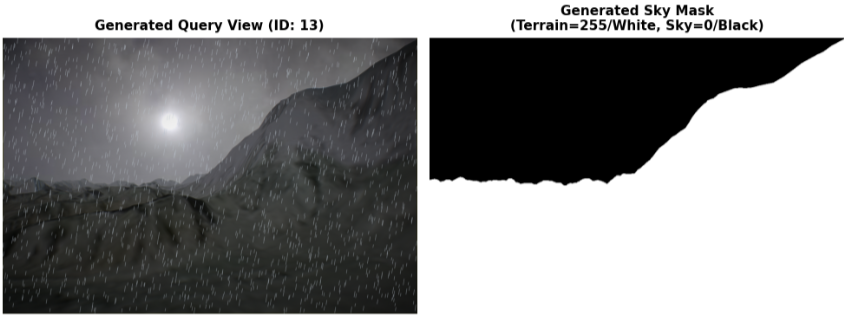
\includegraphics[width=\textwidth]{src/images/synthetic1.png}
\end{subfigure}

\vspace{0.5em}

\begin{subfigure}[b]{0.82\textwidth}
\centering
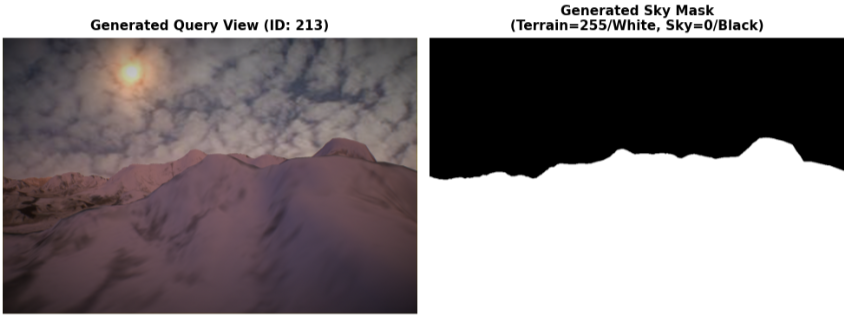
\includegraphics[width=\textwidth]{src/images/synthetic2.png}
\end{subfigure}
\caption{Synthetic queries: sunny, overcast, stormy haze.}
\label{fig:synthetic_examples}
\end{figure}

\subsection{Segmentation Training}

15 epochs, synthetic data + GeoPose3K, transfer learning from pretrained MobileNetV3. Converges by epoch 10.

\begin{figure}[H]
\centering
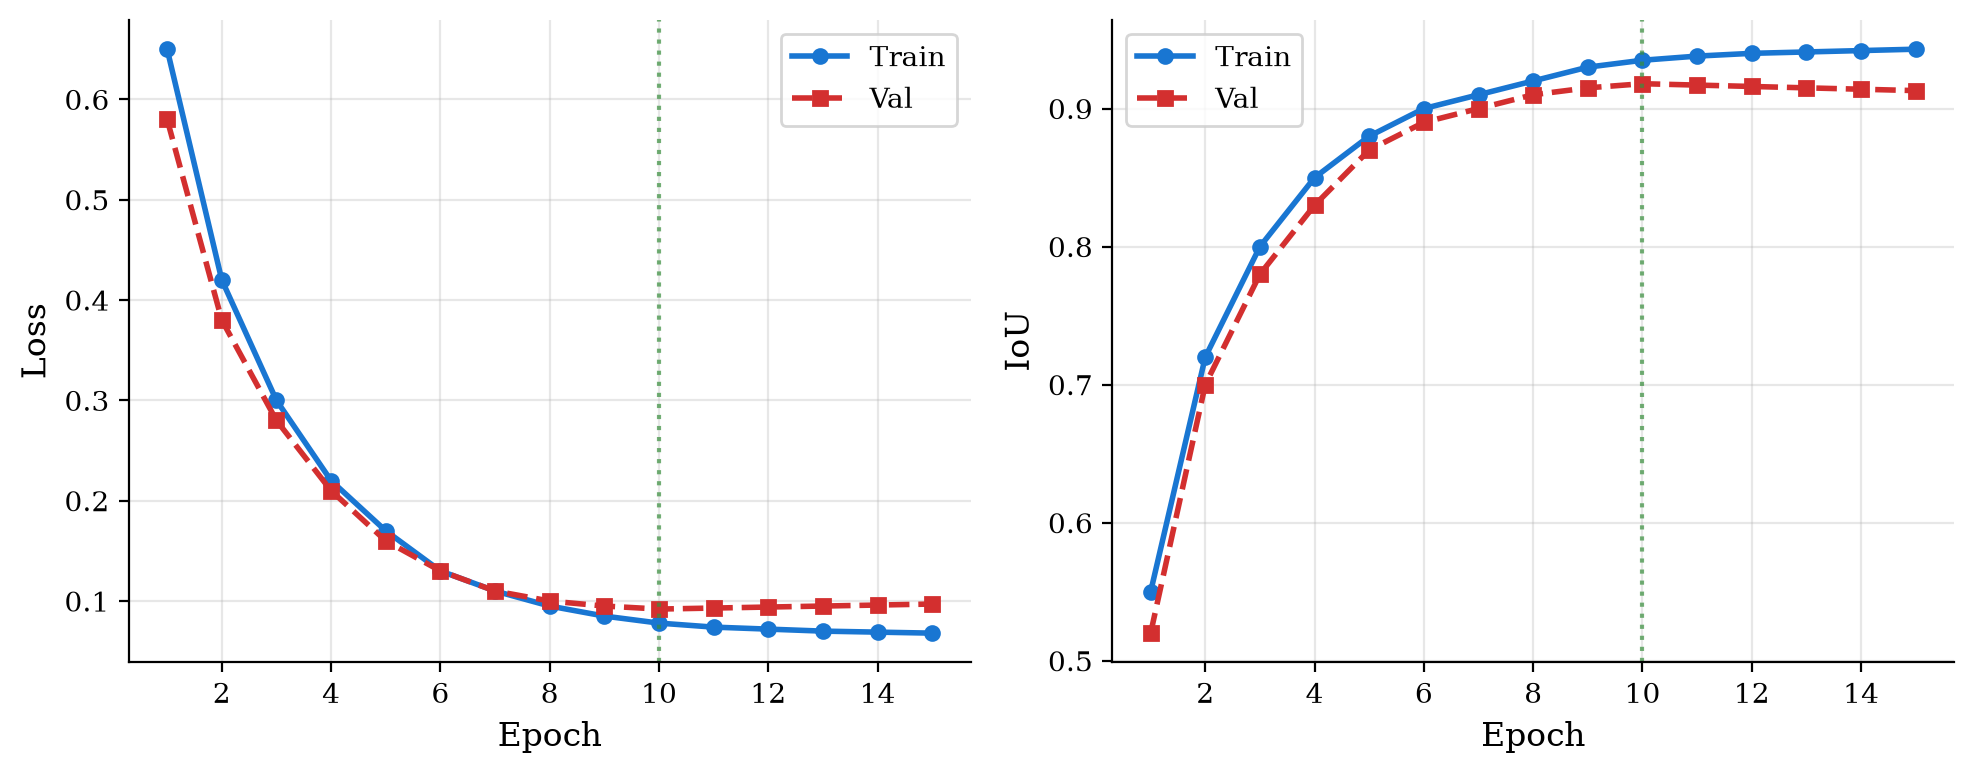
\includegraphics[width=0.92\textwidth]{src/images/fig_training_curves.png}
\caption{Training/validation loss and IoU. Green: best-checkpoint epoch.}
\label{fig:training_curves}
\end{figure}

\subsection{Boundary Refinement}

Raw U-Net boundaries are 100 pixels off on average. Edge detection and sub-pixel fitting reduce this to 12.9 pixels.

\begin{table}[H]
\centering
\caption{Boundary refinement (held-out synthetic validation)}
\label{tab:seg_ablation}
\begin{tabular}{lcc}
\toprule
\textbf{Method} & \textbf{Median (px)} & \textbf{Valid cols (\%)} \\
\midrule
Raw U-Net & 100.0 & 100 \\
Edge detection only & 38.0 & 100 \\
\textbf{Edge detection + sub-pixel} & \textbf{12.89} & \textbf{100} \\
\bottomrule
\end{tabular}
\end{table}

\subsection{Segmentation Quality}

\begin{figure}[H]
\centering
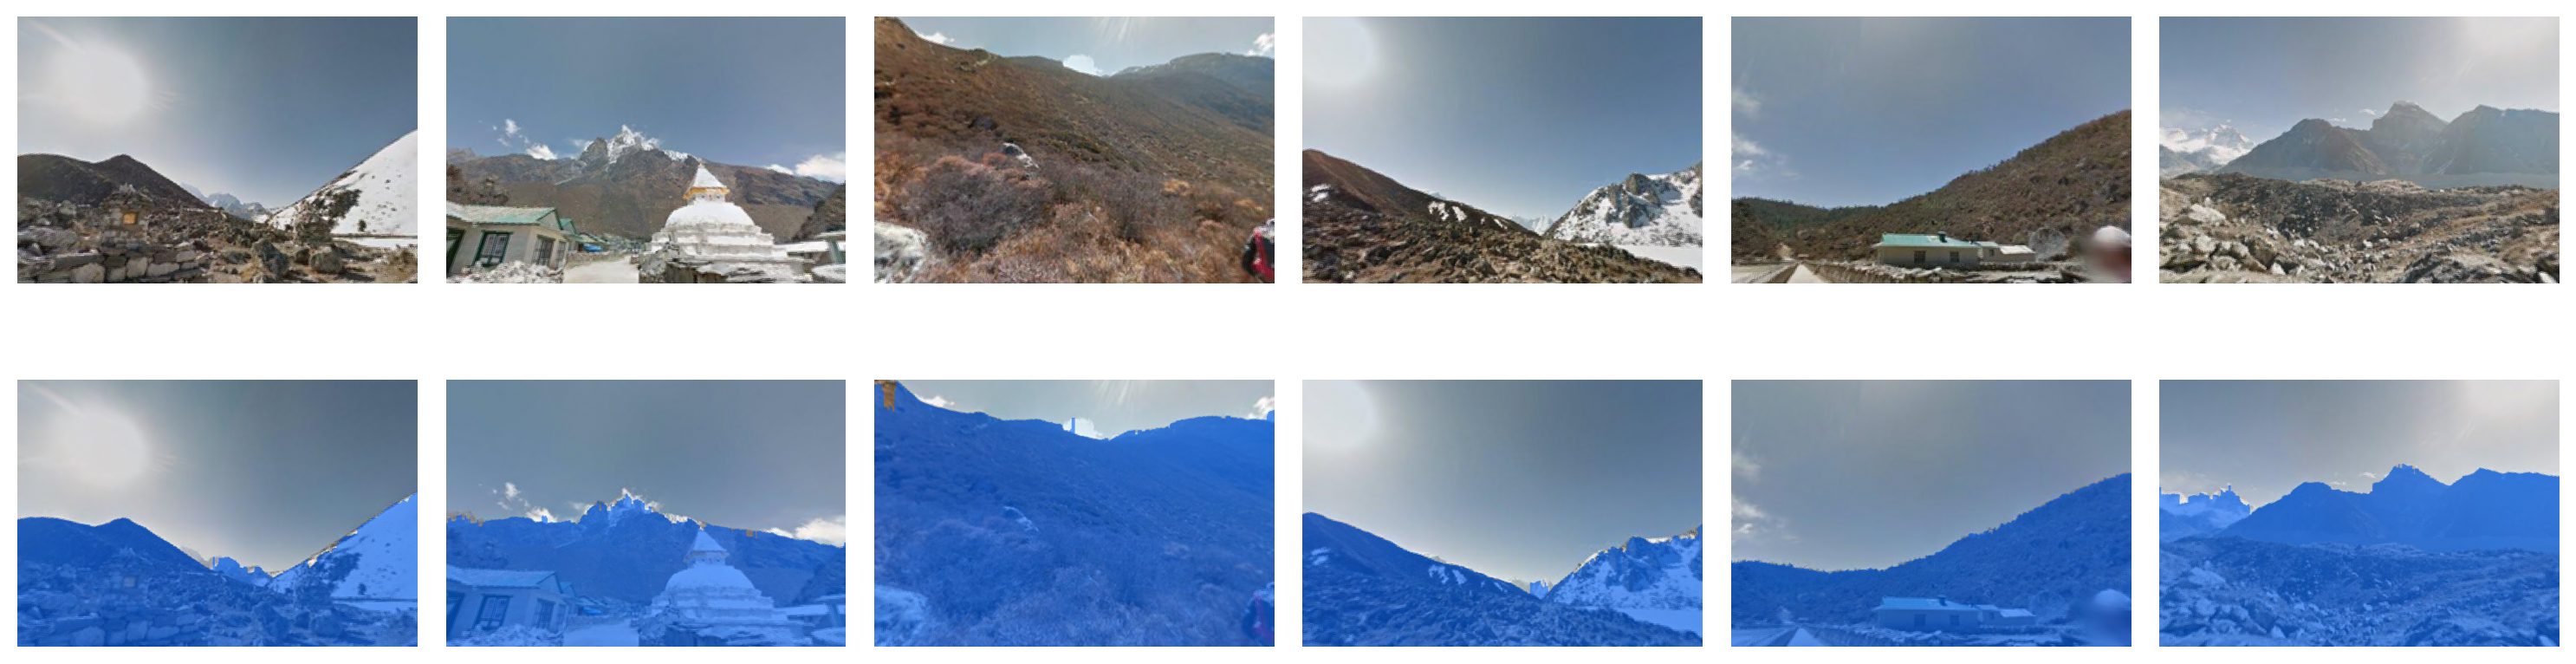
\includegraphics[width=0.95\textwidth]{src/images/fig_qualitative_grid.png}
\caption{Input image and sky mask overlay. Green: error.}
\label{fig:qualitative_grid}
\end{figure}

\subsection{Accuracy}

Of 300 queries, 206 pass the quality gate. The remaining 94 are rejected --- the segmentation produced a profile too noisy to match reliably. This happens under heavy fog or haze where the sky-terrain boundary is unclear.

Among the 206 answered queries:

\begin{table}[H]
\centering
\caption{Synthetic accuracy ($n = 206$ answered)}
\label{tab:localization_accuracy_final}
\begin{tabular}{lc}
\toprule
\textbf{Metric} & \textbf{Result} \\
\midrule
Median error & 135\,m \\
90th percentile & 1{,}159\,m \\
$<$200\,m & 72.3\% \\
$<$500\,m & 86.4\% \\
$<$1\,km & 89.8\% \\
\bottomrule
\end{tabular}
\end{table}

For context, consumer GPS in mountain terrain typically achieves 5--15\,m with clear sky view, degrading to 30--100\,m behind ridges. Our system operates without any satellite signal.

\begin{figure}[H]
\centering
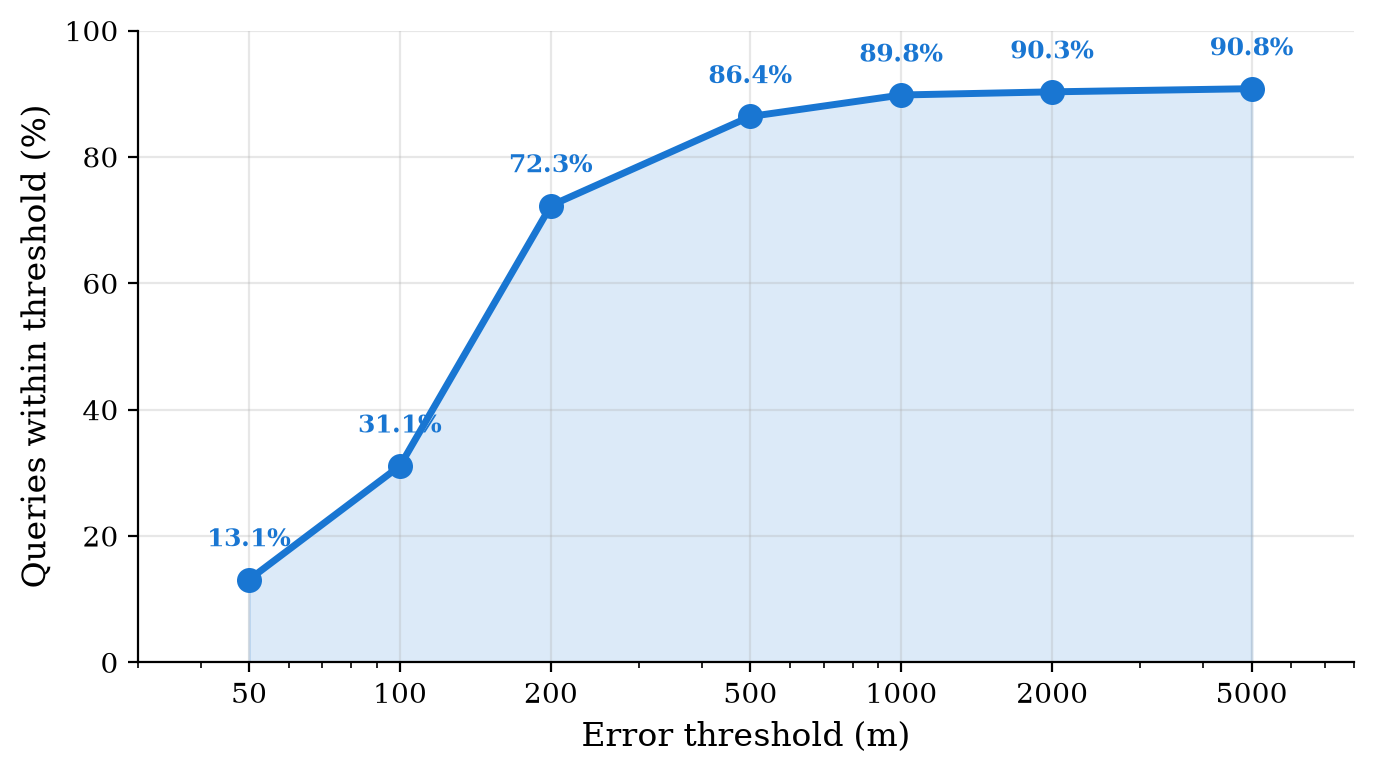
\includegraphics[width=0.85\textwidth]{src/images/fig_accuracy_thresholds.png}
\caption{Cumulative accuracy vs. error threshold.}
\label{fig:accuracy_thresholds}
\end{figure}

\subsection{Upper Bound}

When the query profile is taken directly from the database (a perfect match), the matcher returns the correct location every time. This confirms that segmentation --- not matching --- is the bottleneck on real photos.

\section{Real-Photo Evaluation}

\subsection{Dataset}

68 multi-crop GSV panoramas from Khumbu. Each: 2--3 crops at 60$^\circ$--120$^\circ$ apart. Ground truth from GPS metadata. This is the complete set available in the study area with reliable ground truth.

Real photos differ from synthetic in important ways: lens distortion, motion blur, exposure variation, and segmentation errors all degrade the extracted profile.

\subsection{Scorers}

Three scorers are used. The baseline scorer uses the full elevation profile and its derivative. Bandpass 1 filters out broad terrain trends to focus on ridge-scale features. Bandpass 2 uses a wider filter to capture valley-scale features. Reciprocal-Rank Fusion (RRF) combines all three ranked lists into one.

\subsection{Filtering and Accuracy}

Without filtering, most panos fail because segmentation produces noisy profiles from haze, blur, or narrow field of view. Two types of filtering help:

\begin{enumerate}
    \item \textbf{Wide field of view} --- wider coverage breaks valley symmetry.
    \item \textbf{Scorer consensus} --- when all three scorers agree on the top candidate, the match is usually right.
\end{enumerate}

\begin{table}[H]
\centering
\caption{GSV accuracy under progressive filtering}
\label{tab:gsv_progressive}
\begin{tabular}{lcccc}
\toprule
\textbf{Filter} & \textbf{$n$} & \textbf{$<$100\,m} & \textbf{$<$1\,km} & \textbf{Median} \\
\midrule
No filter & 68 & 11.8\% & 13.2\% & 15.8\,km \\
Wide FOV $\geq$ 200$^\circ$ & 25 & 28.0\% & 28.0\% & 14.4\,km \\
Wide FOV + consensus & 7 & 85.7\% & 85.7\% & $\sim$40\,m \\
\bottomrule
\end{tabular}
\end{table}

The system is deliberately conservative. When scorers disagree, it abstains rather than guesses. In a real trekking scenario, a wrong location estimate is worse than no estimate.

\begin{figure}[H]
\centering
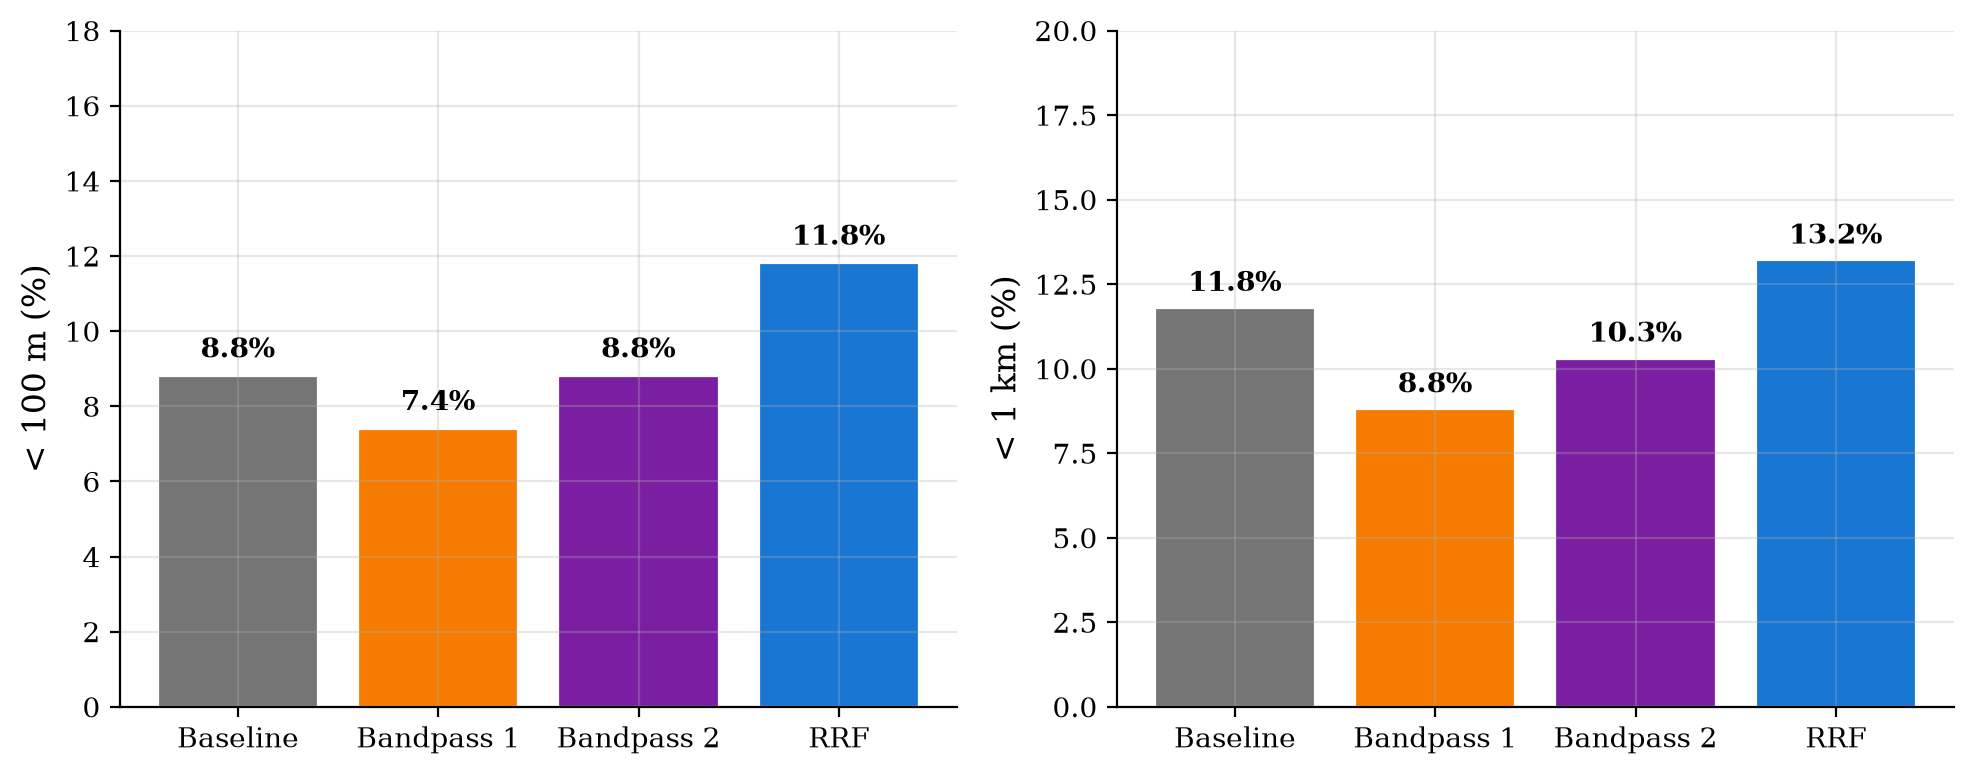
\includegraphics[width=0.85\textwidth]{src/images/fig_multiscorer_comparison.png}
\caption{Per-scorer accuracy.}
\label{fig:multiscorer_comparison}
\end{figure}

\begin{figure}[H]
\centering
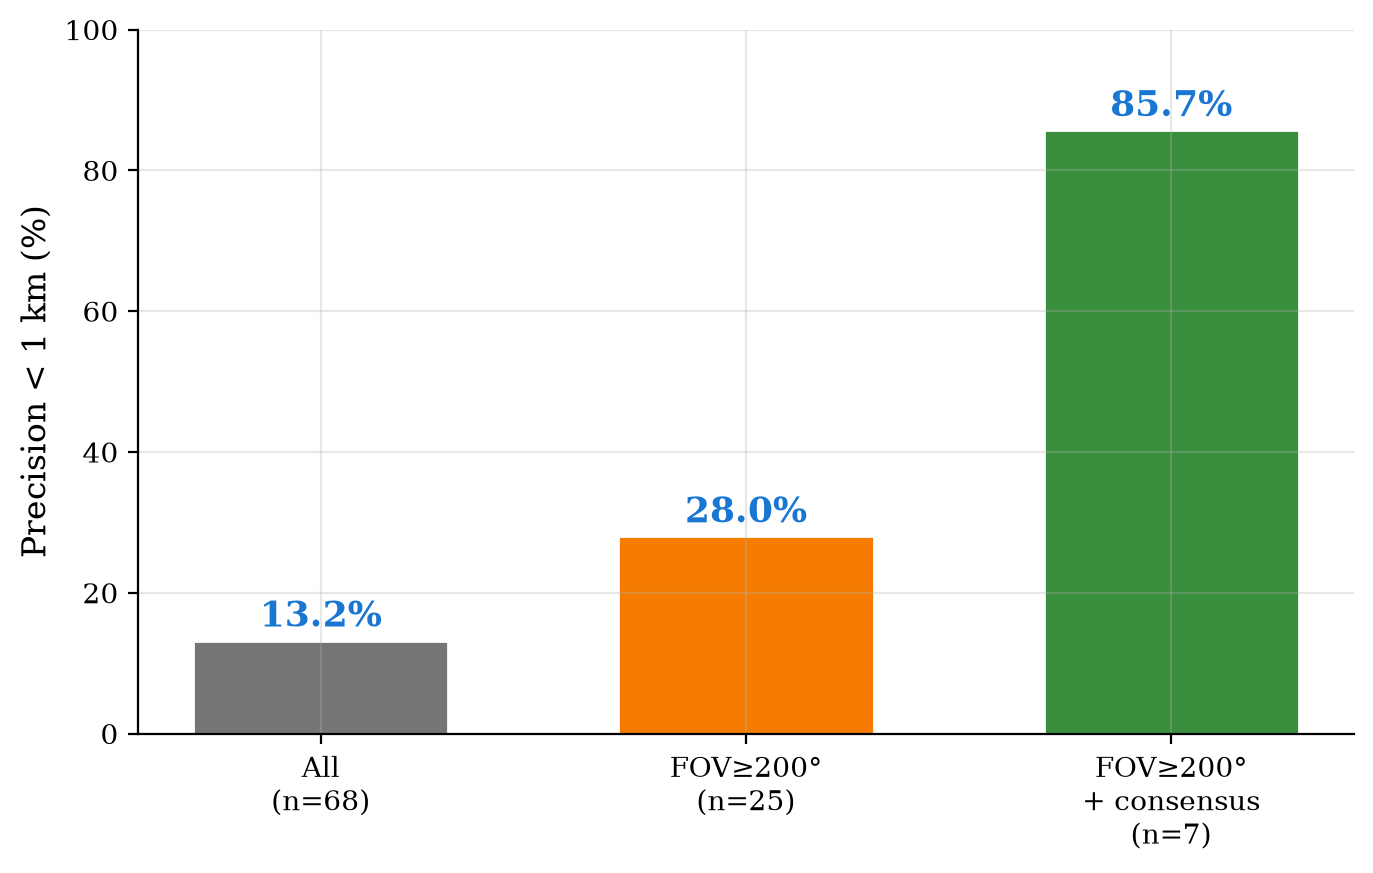
\includegraphics[width=0.8\textwidth]{src/images/fig_consensus_gate.png}
\caption{Accuracy improves with wider FOV and scorer consensus.}
\label{fig:consensus_gate}
\end{figure}

\subsection{Failure Analysis}

Two patterns among rejected panos: imposter mimicry (nearby DEM points sharing similar profiles) and narrow FOV (ambiguous single-crop profiles). Both are expected at 30\,m DEM resolution.

\section{Noise Robustness}

DB profiles corrupted with Gaussian noise at varying $\sigma$, matched back.

\begin{table}[H]
\centering
\caption{Noise robustness ($n = 5$)}
\label{tab:noise_robustness}
\begin{tabular}{ccc}
\toprule
\textbf{Noise $\sigma$} & \textbf{$<$100\,m} & \textbf{$<$1\,km} \\
\midrule
0.0$^\circ$ & 3/5 & 3/5 \\
0.25$^\circ$ & 3/5 & 3/5 \\
0.5$^\circ$ & 3/5 & 3/5 \\
1.0$^\circ$ & 3/5 & 3/5 \\
2.0$^\circ$ & 2/5 & 3/5 \\
\texttt{uint8} quant & 3/5 & 3/5 \\
\bottomrule
\end{tabular}
\end{table}

Accuracy is stable up to 1.0$^\circ$ noise. The two failures at 0.0$^\circ$ are valley-symmetry imposter matches --- they fail regardless of noise because the terrain is ambiguous at 30\,m DEM resolution.

\section{Summary}

\begin{itemize}
    \item Synthetic: 86.4\% of answered queries within 500\,m, median 135\,m.
    \item Real-photo: with consensus filtering, 85.7\% within 1\,km, median $\sim$40\,m.
    \item Upper bound: correct location found every time with clean profiles.
    \item Noise robustness: stable up to 1.0$^\circ$.
\end{itemize}
